% Springer LNCS manuscript -- generated draft, pending author verification.
% Compile with pdflatex (bibliography is inlined as thebibliography).
\documentclass[runningheads]{llncs}

\usepackage[T1]{fontenc}
\usepackage{graphicx}
\usepackage{booktabs}
\usepackage{amsmath}
\usepackage{array}
\usepackage{xcolor}
\usepackage{hyperref}
\renewcommand\UrlFont{\color{blue}\rmfamily}
\urlstyle{rm}

\begin{document}

\title{When the Grader Has a Style: Format-Biased Verifiers
Cause Capability Collapse in Iterative Self-Training of
Small Reasoning Models}

\titlerunning{Format-Biased Verifiers Cause Collapse in Iterative Self-Training}

\author{First Author\inst{1} \and Second Author\inst{1}}
\authorrunning{F. Author and S. Author}
\institute{Ton Duc Thang University, Ho Chi Minh City, Vietnam\\
\email{\{first.author,second.author\}@example.edu}}

\maketitle

\begin{abstract}
Iterative self-training loops of the form generate $\rightarrow$ verify
$\rightarrow$ select $\rightarrow$ train (GVT) are widely used to improve
small language models on mathematical reasoning without human labels, on
the assumption that an automated verifier reliably separates correct from
incorrect solutions. We study what happens when the verifier is a
rule-based checker with a \emph{directional} bias: it rejects correct
solutions written in valid but unexpected formats (false negatives) while
almost never accepting incorrect ones (near-zero false positives). Running
the GVT loop for five rounds on a pooled GSM8K + MATH-500 test set with
\texttt{math-verify} as the verifier and LoRA supervised fine-tuning, we
find that both pass@1 and pass@8 decline monotonically for two model sizes
(Qwen2.5-0.5B and Qwen2.5-1.5B). The degradation is not a plateau or mild
regression: for the 1.5B model pass@1 falls from 50.0\% to 18.6\% and
pass@8 from 72.6\% to 48.6\% over five rounds. Counter-intuitively, the
larger model collapses substantially more than the smaller one. Output
style converges alongside the decline, and the verifier-accepted training
pool shrinks by up to 60\% by the final round. We attribute the effect to a
self-reinforcing shrinking-pool mechanism and argue that a rising pass@1
across rounds is, on its own, insufficient evidence that a self-trained
model is improving when the verifier is rule-based.

\keywords{self-training \and verifier bias \and mathematical reasoning
\and small language models \and model collapse \and pass@k.}
\end{abstract}

\section{Introduction}
\label{sec:intro}

A common recipe for improving the mathematical reasoning of a small
language model (SLM) \emph{without additional human annotation} is to let
the model generate its own solutions, keep those that an automated
verifier judges correct, and fine-tune the model on the kept solutions,
repeating the process for several rounds. We refer to this recipe as the
\emph{Generate--Verify--Train} (GVT) loop. It underlies a family of
methods, including STaR~\cite{ref_star}, ReST~\cite{ref_rest} and
ReST-EM~\cite{ref_restem}, and rejection-sampling fine-tuning
(RFT)~\cite{ref_rft}. Its appeal is that the verifier plays the role of a
teacher that needs only to decide right from wrong; no reference solutions
are required.

Every method in this family rests on an implicit assumption: the verifier
separates correct from incorrect solutions reliably. This assumption is
routinely violated when the verifier is \emph{rule-based} --- the most
common choice for mathematics, because it is cheap, fast, and needs no
training of its own. A rule-based verifier such as
\texttt{math-verify}\footnote{\url{https://github.com/huggingface/math-verify},
version 0.9.0 with antlr4 4.13.2 in this work.}
extracts the final answer from a solution and compares it to the gold
answer after normalisation. It does not read the reasoning, and its
normalisation step never covers every equivalent way of writing an answer.
As a result it produces \emph{false negatives}: it rejects solutions that
are correct but written in a form it does not recognise. Crucially, this
error is \emph{directional}. Because the verifier compares an extracted
final answer against the gold, it almost never accepts a wrong answer --- a
false positive would require an incorrect answer that normalises exactly to
the gold, which is rare. Its errors are therefore overwhelmingly false
negatives, all pushing in one direction.

We measured this bias directly on \texttt{math-verify}
(Section~\ref{sec:verifier}). On GSM8K, whose answers are simple integers,
the false-negative rate on genuinely correct solutions is effectively
zero. On MATH-500, whose answers contain fractions and non-trivial
\LaTeX{}, it rises to roughly 7.8\%, and some individually valid rewrites
--- for instance writing \verb|\dfrac| instead of \verb|\frac| --- are
rejected 100\% of the time even though the numeric value is correct. The
bias is one-sided: we did not observe the verifier accepting incorrect
final answers.

This paper asks a single question: \emph{when a directionally biased
verifier of this kind is used as the filter inside a GVT loop, and the
loop is run for many rounds rather than once, what is the consequence ---
does the model actually improve at reasoning, does it merely learn to
write in the style the verifier prefers, or does it lose capability?}

Prior work has examined one half of this question at a time. Studies of
verifier bias analyse a \emph{single} training round (TinyV~\cite{ref_tinyv};
From Accuracy to Robustness~\cite{ref_robustness}; Imperfect
Verifiers~\cite{ref_imperfect}). Studies of multi-round self-training
either do not characterise the verifier
(ReST-EM~\cite{ref_restem}) or deliberately use an exact, unbiased one
(Teacher-Free Self-Training~\cite{ref_teacherfree}, whose verifier is
defined by exact string equality). To our knowledge, no prior study
combines a \emph{measured, directionally biased} verifier with multi-round
self-training and tracks capability and stylistic drift together.

\paragraph{Contributions.}
\begin{itemize}
\item We run the GVT loop for five rounds with \texttt{math-verify} --- a
real rule-based verifier, not a simulated noise model --- on two model
sizes (Qwen2.5-0.5B-Instruct and Qwen2.5-1.5B-Instruct) and a pooled
GSM8K + MATH-500 test set, and we report pass@1, pass@8, output-style
statistics, and per-problem transition counts at every round.
\item We find that the consequence is not the hypothesised ``style
learning'' with flat capability, but \emph{outright capability collapse}:
pass@1 \emph{and} pass@8 both decline monotonically for both model sizes,
accompanied by stylistic convergence and a shrinking training pool.
\item We report a counter-intuitive secondary finding: collapse severity
\emph{increases} with model size. The 1.5B model (three times the
parameters) degrades far more than the 0.5B model (pass@1 $-63\%$ vs.\
$-12\%$), rather than being more stable.
\end{itemize}

\section{Related Work}
\label{sec:related}

\paragraph{Iterative self-training for reasoning.}
STaR~\cite{ref_star} introduced the generate--filter--retrain loop for
reasoning without hand-written rationales. ReST~\cite{ref_rest} and
ReST-EM~\cite{ref_restem} formalise it as alternating ``grow'' and
``improve'' steps; ReST-EM applies it to MATH and APPS with PaLM-2,
sampling 32 solutions per problem, and reports diminishing test gains after
the first round, plus a one-round regression on APPS that it does not
investigate. RFT~\cite{ref_rft} is the single-round rejection-sampling
special case. All of these treat the correctness signal as trustworthy;
none analyses a verifier that is biased in a fixed direction, and none
tracks output style across rounds.

\paragraph{Verifier and reward error.}
TinyV~\cite{ref_tinyv} measures that a rule-based verifier rejects a large
fraction of correct solutions and \emph{repairs} the verifier with an
auxiliary LLM check, evaluated in a single pass. From Accuracy to
Robustness~\cite{ref_robustness} reports that rule-based verifiers for
mathematical RL achieve only about 86\% recall on average (i.e.\ $\sim$14\%
false negatives), an independent figure consistent with ours, but runs RL
for a few hundred steps within one training phase and does not track how
verifier recall interacts with self-training rounds. Imperfect
Verifiers~\cite{ref_imperfect} gives the most formal noise model: the
verifier flips its decision with fixed probabilities $\rho_0$ (false
accept) and $\rho_1$ (false reject). Its Section~3.1 explicitly notes that
``real-world noise can depend on content, formatting, prompt style'', but
then assumes content-independent fixed rates and studies a single RL round.
We fill exactly the gap it names but does not pursue.

\paragraph{Limits of RL and self-training.}
Yue et al.~\cite{ref_rllimit} show that RL raises pass@1 while the base
model wins at large pass@$k$, i.e.\ RL sharpens an existing distribution
rather than extending capability. Teacher-Free
Self-Training~\cite{ref_teacherfree} runs three sequential self-training
rounds on a free-verifier domain and observes a pass@8 vs.\ pass@64
crossover --- the trained model wins at small sampling budget and loses at
large budget --- concluding that self-training ``amplifies but does not
compound''. Its verifier is exact string equality, with ``zero learned
opinion''; the effect is explained by sharpening alone, with no biased
verifier in play. Our setting differs precisely in that the verifier
\emph{is} biased, and we observe decline at \emph{both} pass@1 and pass@8.

\paragraph{Model collapse.}
Training repeatedly on model-generated data erodes distribution tails and
converges output toward the mean~\cite{ref_collapse}. Classic model
collapse arises when training on the \emph{entire} self-generated
distribution; here we see a related contraction even though we train only
on the subset that a supposedly trustworthy verifier accepted. Qiao et
al.~\cite{ref_selectionbias} argue theoretically that a selector able to
``see'' only a narrow slice of the target distribution becomes itself a
source of bias that accelerates collapse --- the mechanism we observe
empirically.

\paragraph{Single-round verifier-error studies.}
Egashira et al.~\cite{ref_delayplateau} classify verifier errors in
one-round RLVR on synthetic arithmetic and conclude that systematic false
negatives behave like random noise (they slow learning but do not cause
collapse), while false positives cause plateau or collapse. Their
conclusion sounds opposed to ours, and we address it directly in
Section~\ref{sec:discussion}: they study one RLVR phase with a simulated
verifier, whereas the shrinking-training-pool mechanism we identify only
appears under multi-round supervised self-training that re-initialises from
the base model each round.

\paragraph{Summary.}
No prior work combines all three ingredients of our study: a real,
measured, format-biased rule-based verifier; multiple sequential
self-training rounds; and joint tracking of capability (pass@1/pass@$k$)
and output style. Two independent works brush against this gap --- ReST-EM
reports an uninvestigated round-2 regression, and Imperfect Verifiers names
format-dependent noise as out of scope --- which suggests the gap is real
and worth closing.

\section{Setup}
\label{sec:setup}

\subsection{The GVT Loop}
\label{sec:loop}

Each round $t$ of our loop performs four steps.
\begin{description}
\item[Generate.] For every problem in the working set, the current model
samples $k = 8$ solutions (temperature sampling).
\item[Verify.] \texttt{math-verify} (version 0.9.0, antlr4 4.13.2) extracts
the final answer from each solution and compares it to the gold answer.
\item[Select.] Solutions the verifier accepts are kept; all others are
discarded.
\item[Train.] A \emph{fresh} LoRA adapter (rank 16, $\alpha = 32$) is
attached to the \emph{base} model and trained by supervised fine-tuning on
the kept solutions for one epoch. Adapters are \emph{not} accumulated
across rounds: round $t$ starts from the base weights and learns only from
round $t-1$'s accepted pool.
\end{description}
The loop is run for five rounds ($t = 0,\dots,4$), where $t = 0$ is the
untrained base model.

\subsection{The Verifier and Its Directional Bias}
\label{sec:verifier}

Before running the loop we characterised \texttt{math-verify} in two ways.

\emph{Format probe.} We took gold answers from GSM8K and MATH-500 and
re-rendered each in a set of individually valid formats (bare number,
trailing-zero decimal, \verb|\frac|, \verb|\dfrac|, \verb|\tfrac|, boxed,
dollar-delimited, full sentence, with units), then asked the verifier to
grade the re-rendered answer against the original gold. On GSM8K, plain
rewrites are never rejected; \verb|\dfrac| and \verb|\tfrac| are rejected
$200/200$ (the verifier fails to parse the command). On MATH-500,
\verb|\dfrac|/\verb|\tfrac| are rejected $146/146$ ($100\%$),
trailing-zero decimals such as \texttt{0.50} are rejected $59\%$ of the
time, and boxed/dollar-delimited forms are rejected about $20\%$ of the
time.

\emph{False-negative rate on real solutions.} We then took genuinely
correct model-generated solutions (public teacher traces for GSM8K; public
Qwen2.5-7B rollouts for MATH-500) and manually checked, for each solution
the verifier rejected, whether the boxed answer actually matched the gold.
The false-negative rate among correct solutions is $\mathbf{7.8\%}$ on
MATH-500 ($10/128$) and $\mathbf{0\%}$ on GSM8K ($0/200$); the two verifier
presets we tested (\texttt{default} and \texttt{reward}) give identical
counts. Of the ten MATH-500 false negatives, eight are cases where the
verifier extracts the wrong token from a long solution, and two are valid
rewrites it cannot match (\verb|\left( 3, \frac{\pi}{2} \right)| vs.\
\verb|(3, \frac{\pi}{2})|; \verb|6+9i| vs.\ \verb|6 + 9i|). We did not
observe the verifier accepting an incorrect final answer; the error is
one-directional.

\subsection{Models, Data, Training, Metrics}
\label{sec:config}

\emph{Models.} Qwen2.5-0.5B-Instruct and
Qwen2.5-1.5B-Instruct.\footnote{\url{https://huggingface.co/Qwen/Qwen2.5-0.5B-Instruct},
\url{https://huggingface.co/Qwen/Qwen2.5-1.5B-Instruct}.}

\emph{Data.} GSM8K and MATH-500, 500 problems each. Both the \texttt{select}
step and the \texttt{exam} step run on the \emph{test} split; we did not
hold out a separate training split (see Section~\ref{sec:limitations}).
Reported pass rates are pooled over the 1{,}000 problems.

\emph{Training.} LoRA supervised fine-tuning
(\texttt{transformers} + \texttt{peft} + TRL \texttt{SFTTrainer}), one
epoch per round. We use SFT on verifier-accepted solutions rather than
online RL because it matches the select-then-train structure of the loop.

\emph{Metrics, per round.}
(i) pass@1 and pass@8 over the pooled test set;
(ii) style counts over all $8{,}000$ generations per round (500 problems
$\times$ 8 samples $\times$ 2 datasets), for labels including
\texttt{boxed}, \texttt{dfrac}, \texttt{frac}, \texttt{dollar},
\texttt{sentence}, \texttt{assignment}, \texttt{decimal};
(iii) an A/B/C table of per-problem transitions relative to the previous
round: A = newly solved (no accepted sample last round, at least one now),
B = stable/first-attempt-improved, C = lost (had an accepted sample last
round, none now).

\emph{Infrastructure.} A single Kaggle T4 GPU. Each model $\times$ dataset
configuration was run \emph{once}; we did not repeat with multiple seeds
(see Section~\ref{sec:limitations}).

\section{Results}
\label{sec:results}

\subsection{pass@1 and pass@8 Decline Every Round}

Table~\ref{tab:passk} reports pass@1 and pass@8 for both models across the
five rounds; the two verifier presets produced identical values, so a
single column is shown. All four series decline monotonically or nearly so
(the only exception is a $+0.8$-point blip in 0.5B pass@1 at round~1). This
is not random fluctuation around a flat trend.

\begin{table}[t]
\caption{pass@1 and pass@8 over five GVT rounds, pooled GSM8K + MATH-500.
Round 0 is the untrained base model.}
\label{tab:passk}
\centering
\begin{tabular}{llccccc c}
\toprule
Model & Metric & R0 & R1 & R2 & R3 & R4 & $\Delta$ (R0$\to$R4) \\
\midrule
0.5B & pass@1 & 31.1\% & 31.9\% & 29.9\% & 28.9\% & 27.4\% & $-3.7$ pt ($-12\%$) \\
0.5B & pass@8 & 60.5\% & 58.9\% & 56.1\% & 55.5\% & 54.9\% & $-5.6$ pt ($-9\%$) \\
1.5B & pass@1 & 50.0\% & 46.2\% & 44.5\% & 32.4\% & 18.6\% & $\mathbf{-31.4}$ pt ($\mathbf{-63\%}$) \\
1.5B & pass@8 & 72.6\% & 71.5\% & 70.2\% & 63.6\% & 48.6\% & $\mathbf{-24.0}$ pt ($\mathbf{-33\%}$) \\
\bottomrule
\end{tabular}
\end{table}

\begin{figure}[t]
\centering
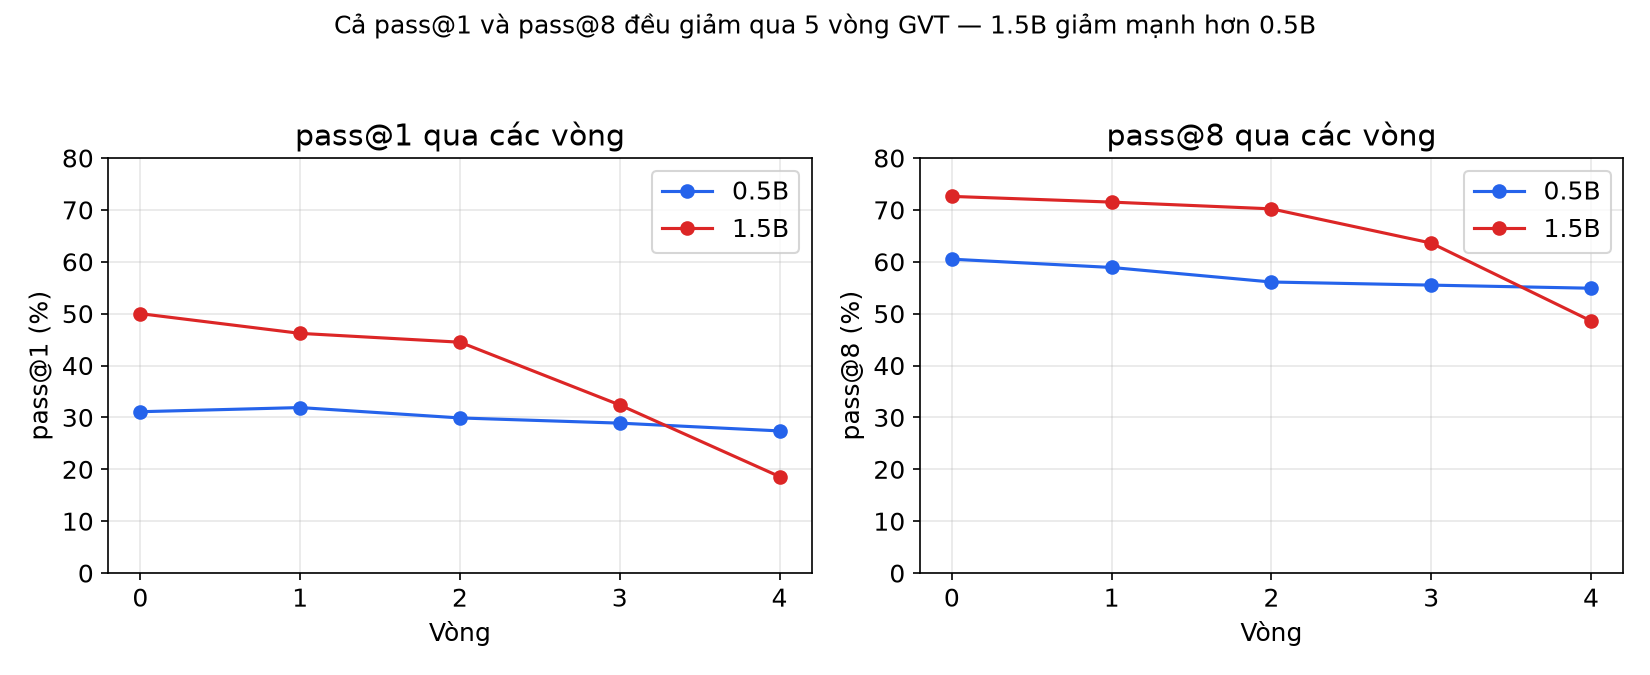
\includegraphics[width=\textwidth]{pass_at_k_by_round.png}
\caption{pass@1 and pass@8 across five rounds for both model sizes. Both
metrics fall for both models; the 1.5B model falls faster and accelerates
in the last two rounds.}
\label{fig:passk}
\end{figure}

The larger model degrades far more than the smaller one --- the opposite of
the stability one might expect from additional capacity. For the 1.5B
model the decline also \emph{accelerates}: most of the pass@1 loss occurs
in rounds 3 and 4.

\subsection{The Accepted Training Pool Shrinks}

Table~\ref{tab:pool} shows the number of verifier-accepted solutions used
for training each round. The pool contracts every round, mildly for the
0.5B model ($-16\%$ by round~4) and sharply for the 1.5B model ($-60\%$).
Because each round trains a fresh adapter on only the previous round's
accepted pool, later rounds learn from a strictly smaller and less diverse
sample.

\begin{table}[t]
\caption{Verifier-accepted solutions used for training, per round.}
\label{tab:pool}
\centering
\begin{tabular}{lccccc c}
\toprule
Model & R0 & R1 & R2 & R3 & R4 & $\Delta$ \\
\midrule
0.5B & 2533 & 2454 & 2339 & 2267 & 2123 & $-16\%$ \\
1.5B & 3962 & 3730 & 3395 & 2638 & 1566 & $\mathbf{-60\%}$ \\
\bottomrule
\end{tabular}
\end{table}

\begin{figure}[t]
\centering
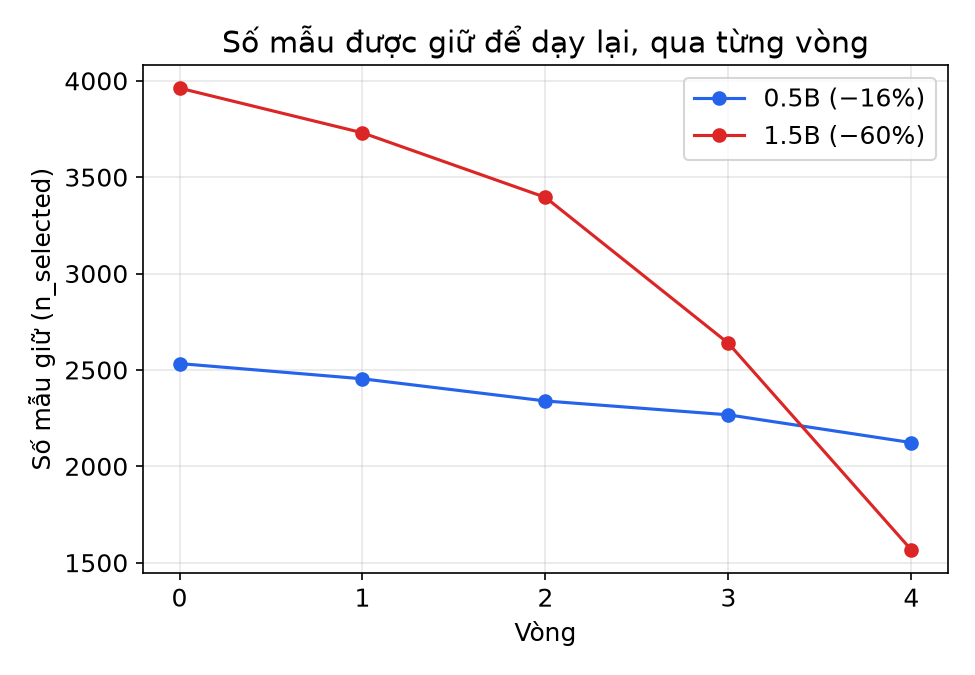
\includegraphics[width=\textwidth]{selected_pool_by_round.png}
\caption{Size of the verifier-accepted training pool by round. The 1.5B
pool collapses in the final two rounds, mirroring the pass-rate curve.}
\label{fig:pool}
\end{figure}

\subsection{Output Style Converges}

For the 1.5B model, output style shifts markedly over the rounds. Boxed
answers (\verb|\boxed{}|) fall from $5{,}608$ to $2{,}693$ occurrences per
round (out of $8{,}000$ generations), while dollar-delimited math
(\verb|$...$|) rises from $1{,}453$ to $3{,}406$ and \verb|\dfrac| usage
grows from $24$ to $241$. For the 0.5B model, by contrast, style counts are
almost flat (boxed $5{,}880 \to 5{,}513$; dollar $1{,}292 \to 1{,}327$).
The model that collapses harder is also the one whose style moves more.

\subsection{Per-Problem Dynamics: Lost Problems Outnumber Gained}

Table~\ref{tab:abc} gives the A/B/C transition counts for the 1.5B model.
Lost problems (C) exceed newly solved problems (A) in all four rounds, and
the gap widens sharply in rounds 3--4, matching the accelerating decline in
Table~\ref{tab:passk}. The aggregate pass rates hide this: a single pass@8
number nets A against C.

\begin{table}[t]
\caption{Per-problem transitions for the 1.5B model, relative to the
previous round. A = newly solved, B = stable, C = lost.}
\label{tab:abc}
\centering
\begin{tabular}{lccc}
\toprule
Round & A (gained) & B (stable) & C (lost) \\
\midrule
1 & 47 & 75 & 58 \\
2 & 53 & 88 & 66 \\
3 & 51 & 60 & \textbf{117} \\
4 & 44 & 43 & \textbf{194} \\
\bottomrule
\end{tabular}
\end{table}

\subsection{Pre-Filter Answer Diversity Increases, It Does Not Collapse}
\label{sec:answer-diversity}

Section~4.3 shows writing \emph{style} converging. A natural follow-up
question is whether the model is also converging onto a single \emph{answer}
per problem --- i.e.\ whether the $k$ raw samples the model produces for one
problem, \emph{before} the verifier ever sees them, become more alike as
training proceeds. We tested this directly on both real Kaggle runs by
extracting each sample's final answer (the same \texttt{extract\_final} +
normalisation routine used for style counting) and measuring, per round: the
mean fraction of distinct normalised answers among the $k=8$ samples for a
problem, and the fraction of problems where all $k$ samples agree on one
answer.

\begin{table}[t]
\caption{Pre-filter answer diversity across $k{=}8$ samples per problem, by
round. A \emph{lower} ``\% all-$k$-agree'' means the model is \emph{less}
consistent about what answer it gives to the same problem.}
\label{tab:answer-diversity}
\centering
\begin{tabular}{lccccc}
\toprule
Model / metric & R0 & R1 & R2 & R3 & R4 \\
\midrule
0.5B, unique answers / $k$ & 0.600 & 0.601 & 0.608 & 0.620 & 0.649 \\
0.5B, \% all-$k$ agree & 10.5\% & 10.8\% & 9.2\% & 9.1\% & 7.3\% \\
1.5B, unique answers / $k$ & 0.443 & 0.482 & 0.543 & 0.634 & 0.712 \\
1.5B, \% all-$k$ agree & \textbf{24.8\%} & 21.4\% & 14.5\% & 6.6\% & \textbf{1.7\%} \\
\bottomrule
\end{tabular}
\end{table}

The result is the \emph{opposite} of the ``the model narrows onto one
preferred output'' framing one might expect from Section~4.3 alone: raw-text
uniqueness among the $k$ samples stays at $\approx\!1.0$ every round for both
models (at temperature $0.8$, $k$ independent samples are almost never
byte-identical regardless of round, so this metric alone is uninformative),
but \emph{answer-level} diversity \emph{rises} monotonically for both models,
sharply so for 1.5B: the fraction of problems on which all 8 samples agree on
one answer falls from $24.8\%$ at round~0 to just $1.7\%$ by round~4. The
model is not converging on a single answer per problem, correct or
incorrect --- it is becoming \emph{less} internally consistent about what
answer it gives to the same problem at all. This is, if anything, a more
direct signature of genuine capability loss than the ``compounding style
bias'' framing we set out to test: a model that still knows how to solve a
problem tends to reach the same (or a similar) answer across repeated
attempts, while a model whose capability is degrading answers increasingly
erratically. It is also consistent with pass@1 falling faster (relatively)
than pass@8 (Table~\ref{tab:passk}): a more scattered answer distribution is
harder to hit on the first try even when a correct answer is still reachable
within $k$ attempts.

\section{Discussion}
\label{sec:discussion}

\subsection{A Self-Reinforcing Shrinking-Pool Mechanism}

In our design each round trains a fresh LoRA adapter from the base model on
exactly the set of solutions the verifier accepted in the previous round.
Because the verifier is directionally biased --- it only rejects, almost
never falsely accepts --- the accepted set at each round is both
\emph{smaller} (Table~\ref{tab:pool}) and \emph{skewed} toward the writing
style the verifier tolerates (Section~4.3). The next round therefore learns
from a pool that is narrower than the one before it, and since that pool is
produced by the previous round's model (already filtered through the biased
verifier), the skew does not cancel out --- it compounds. This is a
self-reinforcing feedback loop closely related to model
collapse~\cite{ref_collapse,ref_selectionbias}, with one important
difference: classic collapse follows from training on the \emph{entire}
self-generated distribution, whereas here the contraction occurs even
though we train only on the verifier-filtered subset. Filtering through a
verifier does not prevent collapse if the filter is itself directionally
biased; it only changes the shape of the collapse from ``regression to the
mean'' into ``contraction toward the verifier's preferred format''.

Note that ``compounding'' here operates on two \emph{different} axes, not
one, and Section~\ref{sec:answer-diversity} shows they move in opposite
directions: output \emph{style} narrows (Section~4.3), while the
\emph{answer content} a sample commits to becomes more scattered, not less.
A single ``the model collapses onto the verifier's preferred output''
story predicts both axes should narrow together; our data rejects that
simple version. A revised reading is that the shrinking, skewed training
pool degrades the model's underlying reliability at solving the problem
(rising answer disagreement across resampled attempts) while separately
pushing surface form toward the verifier's tolerated formats (falling style
diversity) --- two coupled but distinct consequences of training on the same
narrowing pool, not one.

\subsection{Why Does the Larger Model Collapse Harder?}

This is the least intuitive result of the study. The most plausible
hypothesis --- which we do not verify directly here --- is that, under an
identical training configuration (LoRA rank 16, one epoch per round), a
model with more parameters fits the given pool faster and more tightly,
even when that pool is small and skewed. Fitting a progressively narrower
pool more aggressively would accelerate the loss of general behaviour
relative to a smaller model that fits more slowly and thus retains more
general-purpose behaviour each round. The stronger stylistic shift of the
1.5B model (Section~4.3) is consistent with faster fitting. We cannot rule
out an alternative: the same nominal learning rate may have a different
effective magnitude on models of different size. Distinguishing these would
require directly measuring fitting speed per round (training loss on the
kept pool, or output diversity before verifier filtering), which is outside
the scope of the present data.

\subsection{Reconciling with One-Round Studies}

Egashira et al.~\cite{ref_delayplateau} report that systematic false
negatives in one-round RLVR act like random noise and do not cause
collapse. Our result is not in contradiction. They study a single RLVR
phase with a simulated verifier on synthetic arithmetic; the mechanism we
identify --- a training pool that contracts round over round because each
round re-initialises from the base and re-filters through the same biased
verifier --- cannot arise in a single round. Their finding and ours
together suggest that the danger of format-biased false negatives is
specific to the multi-round supervised self-training regime.

\subsection{Practical Implication}

For anyone building a GVT-style pipeline (STaR, ReST-EM, RFT, and
relatives): a pass@1 that rises across rounds is \emph{not} sufficient
evidence that the model is improving. pass@$k$ (retry ability) and
output-style diversity should be tracked in parallel, especially when the
verifier is rule-based --- which, as Section~\ref{sec:verifier} and
\cite{ref_robustness} show, essentially always carries real false
negatives in practice. In our runs, even pass@1 eventually fell; a pipeline
that stopped at round 1 or 2 and looked only at pass@1 would have reported
a near-neutral result and missed an impending collapse.

\section{Limitations}
\label{sec:limitations}

\begin{enumerate}
\item Each model $\times$ dataset configuration was run \emph{once}. The
declines are large and smooth, which makes pure noise unlikely, but we do
not report seed variance.
\item Both \texttt{select} and \texttt{exam} use the GSM8K / MATH-500 test
split; we did not hold out a separate training split. A strict evaluation
would separate them before treating the numbers as final.
\item Only two model sizes (0.5B, 1.5B). Whether ``larger collapses
harder'' continues at 7B+ or reverses somewhere is unknown.
\item Only five rounds. We do not know whether the curve keeps falling,
plateaus, or recovers with more rounds.
\item One verifier (\texttt{math-verify}) and one training method (LoRA
SFT). Whether full fine-tuning or online RL shows the same effect is
untested.
\end{enumerate}

\section{Conclusion}
\label{sec:conclusion}

We measured the consequence of using a directionally biased rule-based
verifier --- one that rejects correct-but-differently-formatted solutions
and almost never accepts incorrect ones --- as the filter in a five-round
GVT self-training loop, on two small mathematical reasoning models. The
outcome matches neither of the two scenarios one might predict in advance
(steady genuine improvement; or flat capability with style drift). Instead,
pass@1 and pass@8 both decline monotonically for both models, with
stylistic convergence and a sharply shrinking training pool, and the
degradation grows with model size. We attribute this to a self-reinforcing
shrinking-pool mechanism that a biased verifier cannot prevent and in fact
shapes. The takeaway for practitioners is concrete: a rising pass@1 across
self-training rounds does not by itself show that a model is improving when
the verifier is rule-based; pass@$k$ and output-style diversity must be
monitored alongside it.

\paragraph{Future work.}
Repeat with multiple seeds; separate train and test splits; add a third,
larger model to test whether ``larger collapses harder'' persists;
directly test the faster-overfitting hypothesis by logging per-round
training loss and pre-filter output diversity.

\begin{credits}
\subsubsection{\ackname}
This work was carried out as an undergraduate research project. No external
funding was received.

\subsubsection{\discintname}
The authors have no competing interests to declare that are relevant to the
content of this article.
\end{credits}

\begin{thebibliography}{99}

\bibitem{ref_imperfect}
Cai, X.-Q., Wang, W., Liu, F., Liu, T., Niu, G., Sugiyama, M.:
Reinforcement Learning with Verifiable yet Noisy Rewards under Imperfect
Verifiers. arXiv:2510.00915 (2025)

\bibitem{ref_gsm8k}
Cobbe, K., Kosaraju, V., Bavarian, M., Chen, M., Jun, H., Kaiser, L.,
Plappert, M., Tworek, J., Hilton, J., Nakano, R., Hesse, C., Schulman, J.:
Training Verifiers to Solve Math Word Problems. arXiv:2110.14168 (2021)

\bibitem{ref_delayplateau}
Egashira, K., Vero, M., Dekoninck, J., D\"orner, F.E., Staab, R., Vechev,
M.: Delay, Plateau, or Collapse: Evaluating the Impact of Systematic
Verification Error on RLVR. arXiv:2605.02909 (2026)

\bibitem{ref_math}
Hendrycks, D., Burns, C., Kadavath, S., Arora, A., Basart, S., Tang, E.,
Song, D., Steinhardt, J.: Measuring Mathematical Problem Solving With the
MATH Dataset. arXiv:2103.03874 (2021)

\bibitem{ref_robustness}
Huang, Y., Zeng, W., Zeng, X., Zhu, Q., He, J.: From Accuracy to
Robustness: A Study of Rule- and Model-based Verifiers in Mathematical
Reasoning. arXiv:2505.22203 (2025)

\bibitem{ref_selectionbias}
Qiao, X., Du, X., Liu, W., Zhang, J., Mai, P., Zhang, M., Pang, Y.:
When Sample Selection Bias Precipitates Model Collapse. arXiv:2606.13732
(2026)

\bibitem{ref_collapse}
Shumailov, I., Shumaylov, Z., Zhao, Y., Papernot, N., Anderson, R., Gal,
Y.: AI models collapse when trained on recursively generated data. Nature
(2024). \doi{10.1038/s41586-024-07566-y}

\bibitem{ref_restem}
Singh, A., Co-Reyes, J.D., Agarwal, R., et al.: Beyond Human Data: Scaling
Self-Training for Problem-Solving with Language Models. arXiv:2312.06585
(2023)

\bibitem{ref_rest}
Gulcehre, C., Le Paine, T., Srinivasan, S., et al.: Reinforced
Self-Training (ReST) for Language Modeling. arXiv:2308.08998 (2023)

\bibitem{ref_teacherfree}
Strozzi, I.L.: Teacher-Free Self-Training Amplifies but Does Not Compound:
A Pass@k Crossover on a Free-Verifier Domain. arXiv:2606.07856 (2026)

\bibitem{ref_tinyv}
Xu, Z., Li, Y., Jiang, F., Ramasubramanian, B., Niu, L., Lin, B.,
Poovendran, R.: TinyV: Reducing False Negatives in Verification Improves RL
for LLM Reasoning. arXiv:2505.14625 (2025)

\bibitem{ref_rft}
Yuan, Z., Yuan, H., Li, C., Dong, G., Lu, K., Tan, C., Zhou, C., Zhou, J.:
Scaling Relationship on Learning Mathematical Reasoning with Large Language
Models. arXiv:2308.01825 (2023)

\bibitem{ref_rllimit}
Yue, Y., Chen, Z., Lu, R., Zhao, A., Wang, Z., Yue, Y., Song, S., Huang,
G.: Does Reinforcement Learning Really Incentivize Reasoning Capacity in
LLMs Beyond the Base Model? arXiv:2504.13837 (2025)

\bibitem{ref_star}
Zelikman, E., Wu, Y., Mu, J., Goodman, N.D.: STaR: Bootstrapping Reasoning
With Reasoning. arXiv:2203.14465 (2022)

\end{thebibliography}

\end{document}
